\documentclass[11pt]{article}

\usepackage[left=1.25in,top=1.25in,right=1.25in,bottom=1.25in,head=1.25in]{geometry}
\usepackage{amsfonts,amsmath,amssymb,amsthm}
\usepackage{graphicx}
\usepackage{subfigure}
\usepackage{hyperref}
\hypersetup{hidelinks,
	colorlinks=true,
	allcolors=black,
	pdfstartview=Fit,
	breaklinks=true}
\title{Summary and discussion of: ``The Implicit Regularization of Stochastic Gradient Flow for Least Squares`` \\
%% replace wih paper title 
\large Journal club report}

\author{Yukun Xie}
%% replace with your names
\date{Dec. 10, 2021}

\begin{document}
\maketitle

\section{Summary} \label{Summary}

In this section, we will firstly briefly introduce content of the paper in Subsection \ref{Intro}. Then we will go through the methods to be talked about in Subsection \ref{Methods}. Both the solution path given in the related paper and our derivations of the formula will be included. The risk and coefficient bounds we talked about will be covered in Subsection \ref{Bounds}. We also present some examples of the SGF using the formula we derive in Subsection \ref{Example} before Section \ref{Results}.

\subsection{Introduction} \label{Intro}

The paper intends to study the Stochastic Differential Equation (SDE), which has the same moments as the Mini-batch Stochastic Gradient Descent (SGD). The authors view the SDE as a continuous version of the SGD and derive the solutions to the SDE in different conditions. We will name the solutions as Stochastic Gradient Flow (SGF).

The paper mainly discuss three things : 

\begin{enumerate}
    \item the relationship between the  SGD and the SGF; 
    
    \item the implicit regularization of the two methods and similarities to the $l_2$ norm
    
    \item the performance of the methods.
\end{enumerate}

Looking back into the contents of MATH5472 course, the paper's contents can also be related to what we have learned before. We have studied the similarities between the Full-batch Gradient Descent and Gradient Flow. We also learnt about the implicit regularization of Gradient Flow and Ridge Regression. So all these methods are linked, and they will be summarized and compared together in this report.

\subsection{Methods and their solutions} \label{Methods}
\begin{equation}
\underset{\beta}{\operatorname{min}} \frac{1}{2 n}\|y-X \beta\|_{2}^{2} .
\end{equation}

The methods in this subsection will all focused on solving the above problem. Here we have $n$ observations of the $p$-dimensional data $X_{n \times p}$ and its response $y_{n \times 1}$. We will cover all the related methods to be compared in Section \ref{Results}.

\subsubsection{Ridge Regression}

The Ridge Regression's objective function will minimize the sum of squared residual plus a penalty term on the $\beta$. The penalty term is a $l_2$ norm of $\beta$ times the constant value $\lambda$.

\begin{equation}
    \sum_{i=1}^{n}\left(y_{i}-\sum_{j=1}^{p} x_{i j} \beta_{j}\right)^{2}+\lambda \sum_{j=1}^{p} \beta_{j}^{2} ,
\end{equation}
then we will have the solution path of $\hat{\beta}(\lambda)$ as
\begin{equation}
\label{eq:3}
    \hat{\beta}(\lambda)=\left(X^{T} X+n \lambda I\right)^{-1} X^{T} y .
\end{equation}

\subsubsection{Gradient Descent and Stochastic Gradient Descent}  
We directly put the formula \ref{eq:4} and \ref{eq:5} below because GD and SGD are well known.
\begin{equation}
\label{eq:4}
    % \begin{aligned}
    \beta^{(k)} =\beta^{(k-1)}+\frac{\epsilon}{n} \cdot X^{T}\left(y-X \beta^{(k-1)}\right) ,
    % \end{aligned}
\end{equation}

\begin{equation}
\label{eq:5}
    % \begin{aligned}
    \beta^{(k)} =\beta^{(k-1)}+\frac{\epsilon}{m} \cdot X_{\mathcal{I}_{k}}^{T}\left(y_{\mathcal{I}_{k}}-X_{\mathcal{I}_{k}} \beta^{(k-1)}\right) .
    % \end{aligned}
\end{equation}

\subsubsection{Gradient Flow} 

\begin{equation}
\label{eq:6}
    \displaystyle d \beta^{\operatorname{gf}}(t)=\frac{1}{n} X^{T}(y-X \beta(t)) d t ,
\end{equation}

\begin{equation}
\label{eq:7}
    \hat{\beta}^{\operatorname{gf}}(t)=\left(X^{T} X\right)^{+}\left(I-\exp \left(-t X^{T} X / n\right)\right) X^{T} y .
\end{equation}

We use the formula in \cite {ali2020implicit}. The $t$ in formula \ref{eq:7} will be equal to the  $1 / \lambda$ in formula \ref{eq:3} when comparing the two methods.



\subsubsection{Stochastic Gradient Flow : the Stochastic Differential Equation (SDE)}  

The SDE of Stochastic Gradient Flow will be similar to the equation \ref{eq:6}, which will add a term representing the moment function of SGD. The $d W(t)$ is a Brownian motion and can be view as $N(0,d t)$,

\begin{equation}
    \displaystyle d \beta^{\operatorname{sgf}}(t)=\frac{1}{n} X^{T}(y-X \beta(t)) d t+Q_{\epsilon}(\beta(t))^{1 / 2} d W(t) .
\end{equation}

    \begin{enumerate}
        \item Continuous Solution to the SDE
        
        The formula in  \cite {ali2020implicit} is given as
        \begin{equation}
        \label{eq:9}
            \begin{aligned}
            \hat{\beta}^{\operatorname{sgf}}(t)&=\hat{\beta}^{\operatorname{gf}}(t) \\
            &\quad+\exp (-t \hat{\Sigma}) \cdot \int_{0}^{t} \exp (\tau \hat{\Sigma}) Q_{\epsilon}\left(\hat{\beta}^{\operatorname{sgf}}(\tau)\right)^{1 / 2} d W(\tau) ,
            \end{aligned}
        \end{equation}
        and we can approximate the expectation of the second term in formula \ref{eq:9} and decompose the $\hat{\Sigma}=\frac{X^TX}{n}=U Diag(D) U^T$ to get our solution path as :
        \begin{equation}
        \label{eq:10}
            \begin{aligned}
            \hat{\beta}^{\operatorname{sgf}}(t)&=\left(X^{T} X\right)^{+}\left(I-\exp \left(-t X^{T} X / n\right)\right) X^{T} y  \\
            &\quad+\exp (-t \hat{\Sigma}) \cdot \int_{0}^{t} \exp (\tau \hat{\Sigma}) Q_{\epsilon}\left(\hat{\beta}^{\operatorname{sgf}}(\tau)\right)^{1 / 2} d W(\tau) \\
            &=\frac{1}{n} U \operatorname{diag}\left(D^{-1}-D^{-1} \exp (-t D)\right) U^{T} X^{T} y \\
            &\quad+U \operatorname{diag}\left(e^{-t D}\right) U^{T} \cdot \int_{0}^{t} U \operatorname{diag}\left(e^{\tau D}\right) U^{T} Q_{\epsilon}\left(\hat{\beta}^{\operatorname{sgf}}(\tau)\right)^{1 / 2} d W(\tau) \\
            &=\frac{1}{n} U \operatorname{diag}\left(D^{-1}-D^{-1} \exp (-t D)\right) U^{T} X^{T} y \\
            &\quad+U  \cdot \operatorname{diag}\left( \int_{0}^{t}  e^{(\tau-t) D} d W(\tau)  \right) U^{T} Q_{\epsilon}\left(\hat{\beta}^{\operatorname{sgf}}(\tau)\right)^{1 / 2} \\
            &=\frac{1}{n} U \operatorname{diag}\left(D^{-1}-D^{-1} \exp (-t D)\right) U^{T} X^{T} y \\
            &\quad+Q_{\epsilon}\left(\hat{\beta}^{\operatorname{sgf}}(\tau)\right)^{1 / 2} 
            \cdot \operatorname{diag}\left( \sum_{k=1}^{t/\epsilon}  e^{(k\epsilon-t) D} z_k  \right) 
            ,
            \end{aligned}
        \end{equation}
        where $z_k \sim N(0,\epsilon)$.
        
        \item Euler discretization to the SDE (Non-constant covariance)
        
        By setting the $Q_{\epsilon}\left(\hat{\beta}^{\operatorname{sgf}}(\tau)\right)^{1 / 2} = \left(\epsilon \operatorname{Cov}_{\mathcal{I}}\left(\frac{1}{m} X_{\mathcal{I}}^{T}\left(y_{\mathcal{I}}-X_{\mathcal{I}} \beta\right)\right)\right)^{1 / 2}$, we have the discrete solution as

        
        \begin{equation}
        \label{eq:11}
            \begin{aligned}
            \hat{\beta}^{(k)}=& \hat{\beta}^{(k-1)}+\frac{\epsilon}{n} \cdot X^{T}\left(y-X \hat{\beta}^{(k-1)}\right) \\
            &+\epsilon \cdot \operatorname{Cov}_{\mathcal{I}}^{1 / 2}\left(\frac{1}{m} X_{\mathcal{I}}^{T}\left(y_{\mathcal{I}}-X_{\mathcal{I}} \hat{\beta}^{(k-1)}\right)\right) z_{k} \\
            =& \hat{\beta}^{(k-1)}+\frac{\epsilon}{n} \cdot X^{T}\left(y-X \hat{\beta}^{(k-1)}\right) \\
            &+\epsilon \cdot \left(\frac{1}{m}\operatorname{Cov}_{\mathcal{I}} \left( X_{\mathcal{I}}^{T}\left(y_{\mathcal{I}}-X_{\mathcal{I}} \hat{\beta}^{(k-1)}\right)\right)\right)^{1 / 2} z_{k} ,
            \end{aligned}
        \end{equation}
        
        where $z_k \sim N(0,I)$.
        
        \item Euler discretization to the SDE (Constant covariance)
        
        By setting the $Q_{\epsilon}\left(\hat{\beta}^{\operatorname{sgf}}(\tau)\right)^{1 / 2} = \left(\frac{\epsilon}{m} \cdot \hat{\Sigma}\right)^{1 / 2}$, we have the discrete solution as

        
        \begin{equation}
        \label{eq:12}
            \begin{aligned}
            \hat{\beta}^{(k)} &= \hat{\beta}^{(k-1)}+\frac{\epsilon}{n} \cdot X^{T}\left(y-X \hat{\beta}^{(k-1)}\right) 
            +\epsilon \left(\frac{1}{m} \cdot \hat{\Sigma}\right)^{1 / 2} z_{k} \\
            &= \hat{\beta}^{(k-1)}+\frac{\epsilon}{n} \cdot X^{T}\left(y-X \hat{\beta}^{(k-1)}\right) 
            +\epsilon U D^{1/2} U^T z_{k}
            ,
            \end{aligned}
        \end{equation}
        
        where $z_k \sim N(0,I)$.
    \end{enumerate}


\subsection{Risk and Coefficient Bounds} \label{Bounds}

The Bayes risk bounds of Ridge Regression and Gradient Flow are directly from \cite{ali2019continuous}. 

\begin{equation}
\label{eq:bound}
    \begin{aligned}
    &\operatorname{Risk}\left(\hat{\beta}^{\operatorname{sgf}}(t) ; \beta_{0}\right) \leq \operatorname{Bias}^{2}\left(\hat{\beta}^{\operatorname{ridge}}(1 / t) ; \beta_{0}\right) \\
    &+1.6862 \cdot \operatorname{Var}_{\eta}\left(\hat{\beta}^{\text {ridge }}(1 / t)\right)+\epsilon \cdot \frac{n}{m} \sum_{i=1}^{p} \mathbb{E}_{\eta} \nu_{i}(t)
    \end{aligned}
\end{equation}

The coefficient bounds have not been implemented in the simulation, so we only know that the coefficient of SGF will not behave like the bound given in the paper.

\subsection{Examples of the SGF} \label{Example}

To illustrate the SGF algorithm, we choose the continuous solution and discrete solution of the SDE. We use the formula \ref{eq:10} and \ref{eq:11} to implement the algorithm. Since in this simulation, we keep the covariance unconstant along the solution path, the diffusion coefficient is set to $Q_{\epsilon}\left(\hat{\beta}^{\operatorname{sgf}}(\tau)\right)= \left(\epsilon \operatorname{Cov}_{\mathcal{I}}\left(\frac{1}{m} X_{\mathcal{I}}^{T}\left(y_{\mathcal{I}}-X_{\mathcal{I}} \beta\right)\right)\right)$. The approximation of $\operatorname{Cov}_{\mathcal{I}} \left( X_{\mathcal{I}}^{T}\left(y_{\mathcal{I}}-X_{\mathcal{I}} \hat{\beta}^{(k-1)}\right)\right)$ is as follows :
        
\begin{equation}
\label{eq:cov}
    \begin{aligned}
    \operatorname{Cov}_{\mathcal{I}} \left( X_{\mathcal{I}}^{T}\left(y_{\mathcal{I}}-X_{\mathcal{I}} \hat{\beta}^{(k-1)}\right)\right) &= \operatorname{Cov}_{\mathcal{I}} \left( \delta f(\cdot) \right) \\
    &= E\left[ \delta f^2(\cdot) \right] - E\left[ \delta f(\cdot) \right]^2 \\
    &= \frac{1}{m} \sum_{i=1}^m \left[ X_i^{T}\left(y_i-X_i \hat{\beta}^{(k-1)}\right)\right] \left[ X_i^{T}\left(y_i-X_i \hat{\beta}^{(k-1)}\right)\right]^T \\
    &+ \left[ \frac{1}{m} \sum_{i=1}^m X_i^{T}\left(y_i-X_i \hat{\beta}^{(k-1)}\right)\right]^2 .
    \end{aligned}
\end{equation}

Then is our settings of the simulation. $n=100$, $p=10$. Number of lambdas for equation is \ref{eq:10} $nt=100$, the range is $[1/100^{max(eigen(\hat{\Sigma}))},10]$. Number of steps for equation \ref{eq:11} is $nk=1000$ and learning rate is set to $\epsilon=0.01$ so that $nk \times \epsilon = 10$. The $\beta \sim N(0,\sigma^2_{\beta} I)$, $X \sim N(0, I)$ and $y \sim N(X\beta,\sigma^2_{n} I)$. We set $\sigma^2_{\beta} = \sigma^2_{n} = 0.5$, and the evolution of the coefficient $\beta$ will be

\begin{figure}[p]
\centering
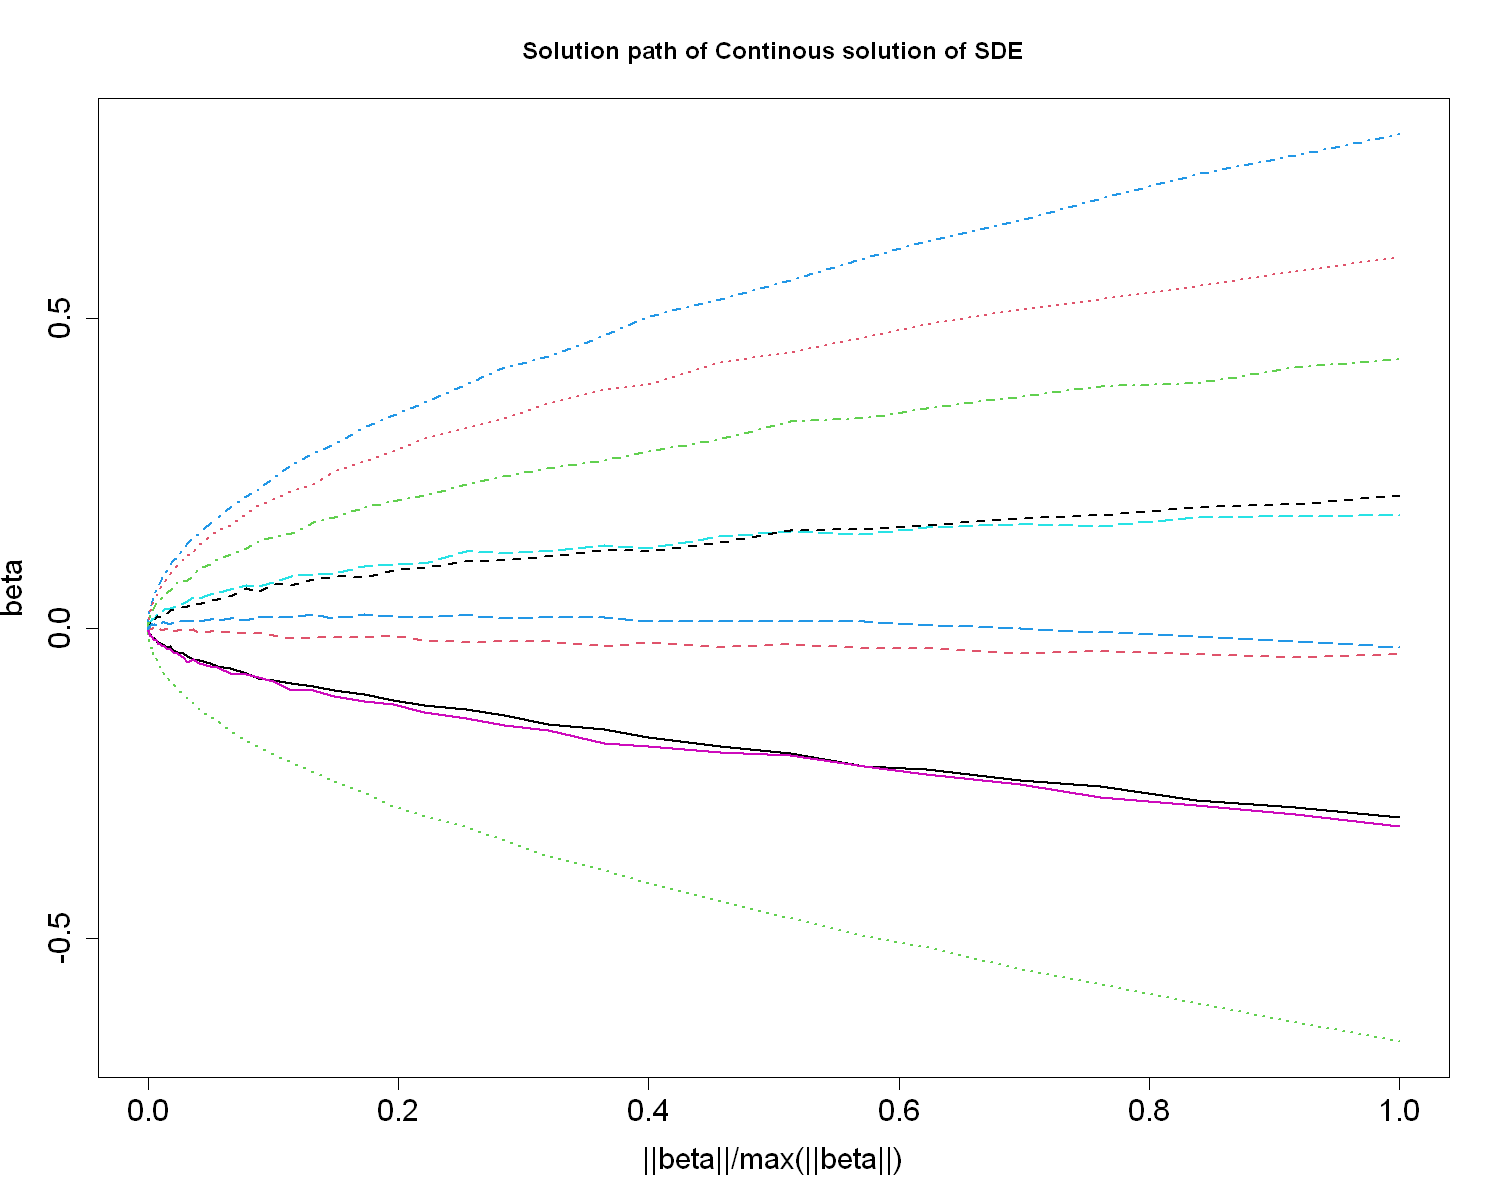
\includegraphics[width=0.75\linewidth]{fig1.png}
\caption{Continuous solution of SDE}
\label{fig:Conti_sde}
\end{figure}

\begin{figure}[p]
\centering
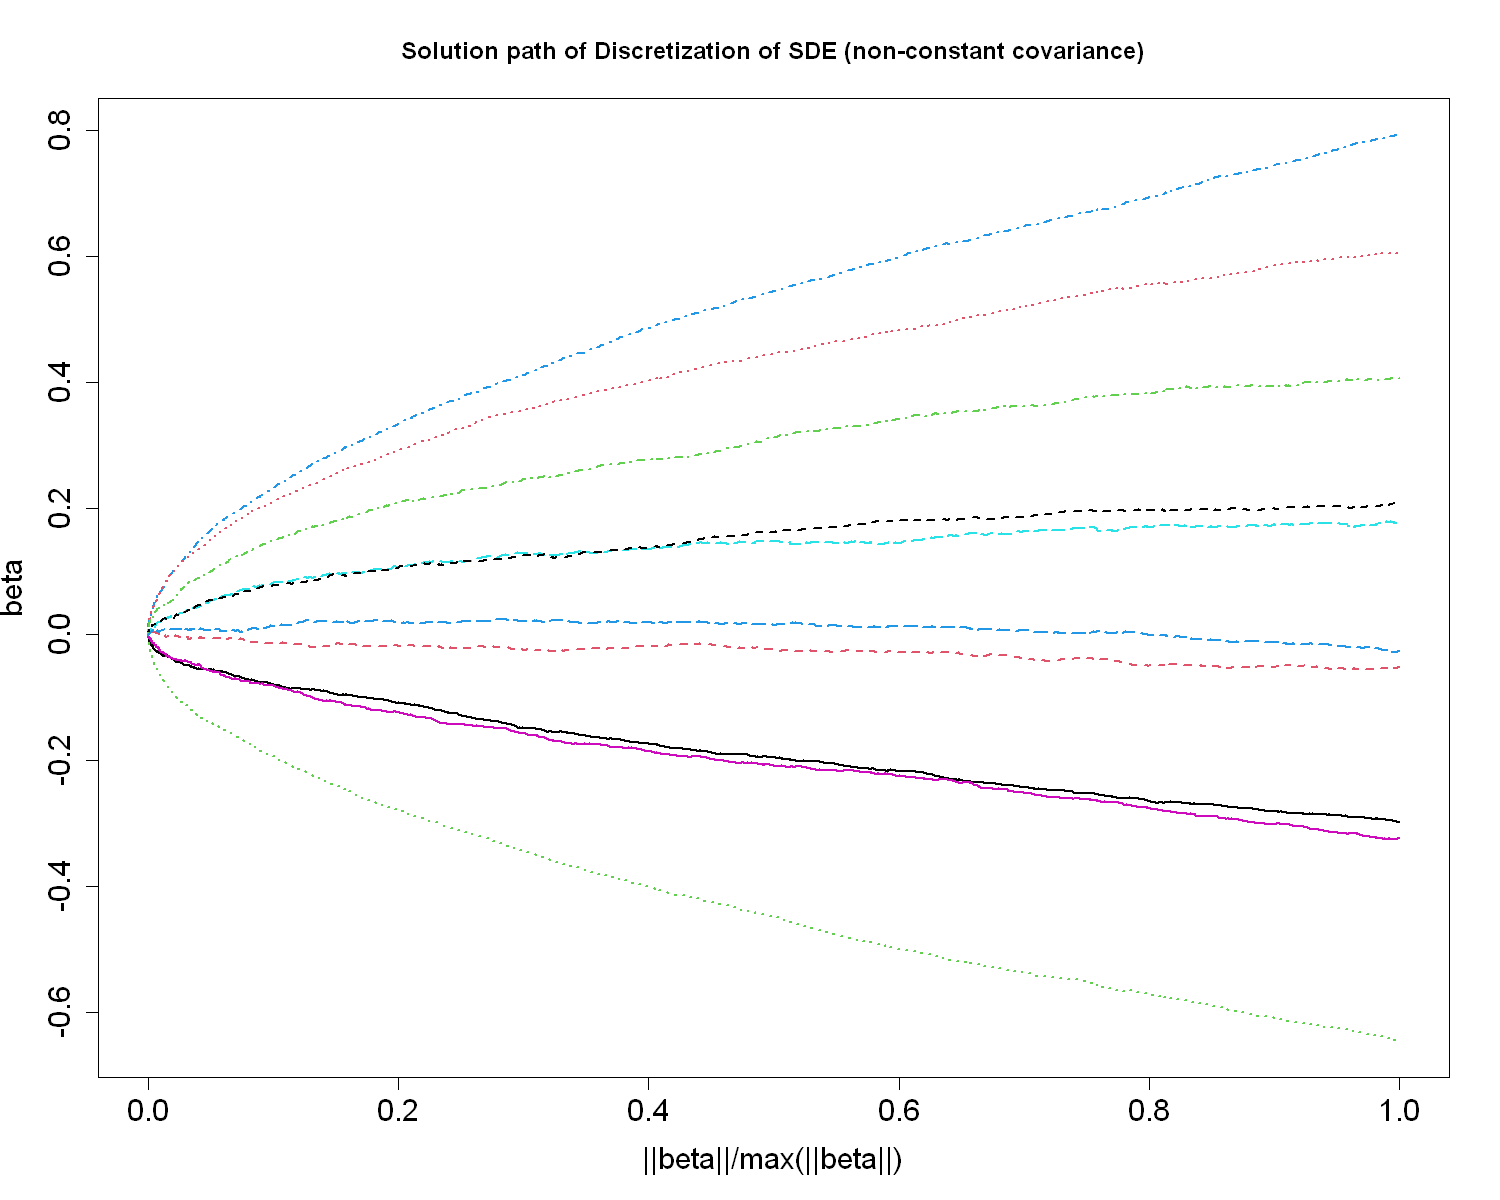
\includegraphics[width=0.75\linewidth]{fig2.png}
\caption{Discrete solution of SDE}
\label{fig:C_sde}
\end{figure}

From Figure \ref{fig:Conti_sde} and Figure \ref{fig:C_sde}, we can find that our algorithm works and results of our two solutions are roughly the same. We further make comparisons between the methods in Section \ref{Results}.

\newpage

\section{Result and Discussion} \label{Results}

In this section we will present three simulations to reproduce the Fig.1, Fig.2 and Fig.4's experiments in \cite{ali2020implicit}. We will also add some more methods into the simulation to connect to what we have learned before.

\subsection{Simulation I}

We will compare the methods we mentioned in Subsection \ref{Methods} before. Here we add additional settings that number of lambdas for ridge is $nlam=50$ and the range of $1/\lambda$ is $[1/100^{max(eigen(\hat{\Sigma}))}, 10]$. The other settings of the simulation is the same as Subsection \ref{Example}. 

\begin{figure}[h]
\centering
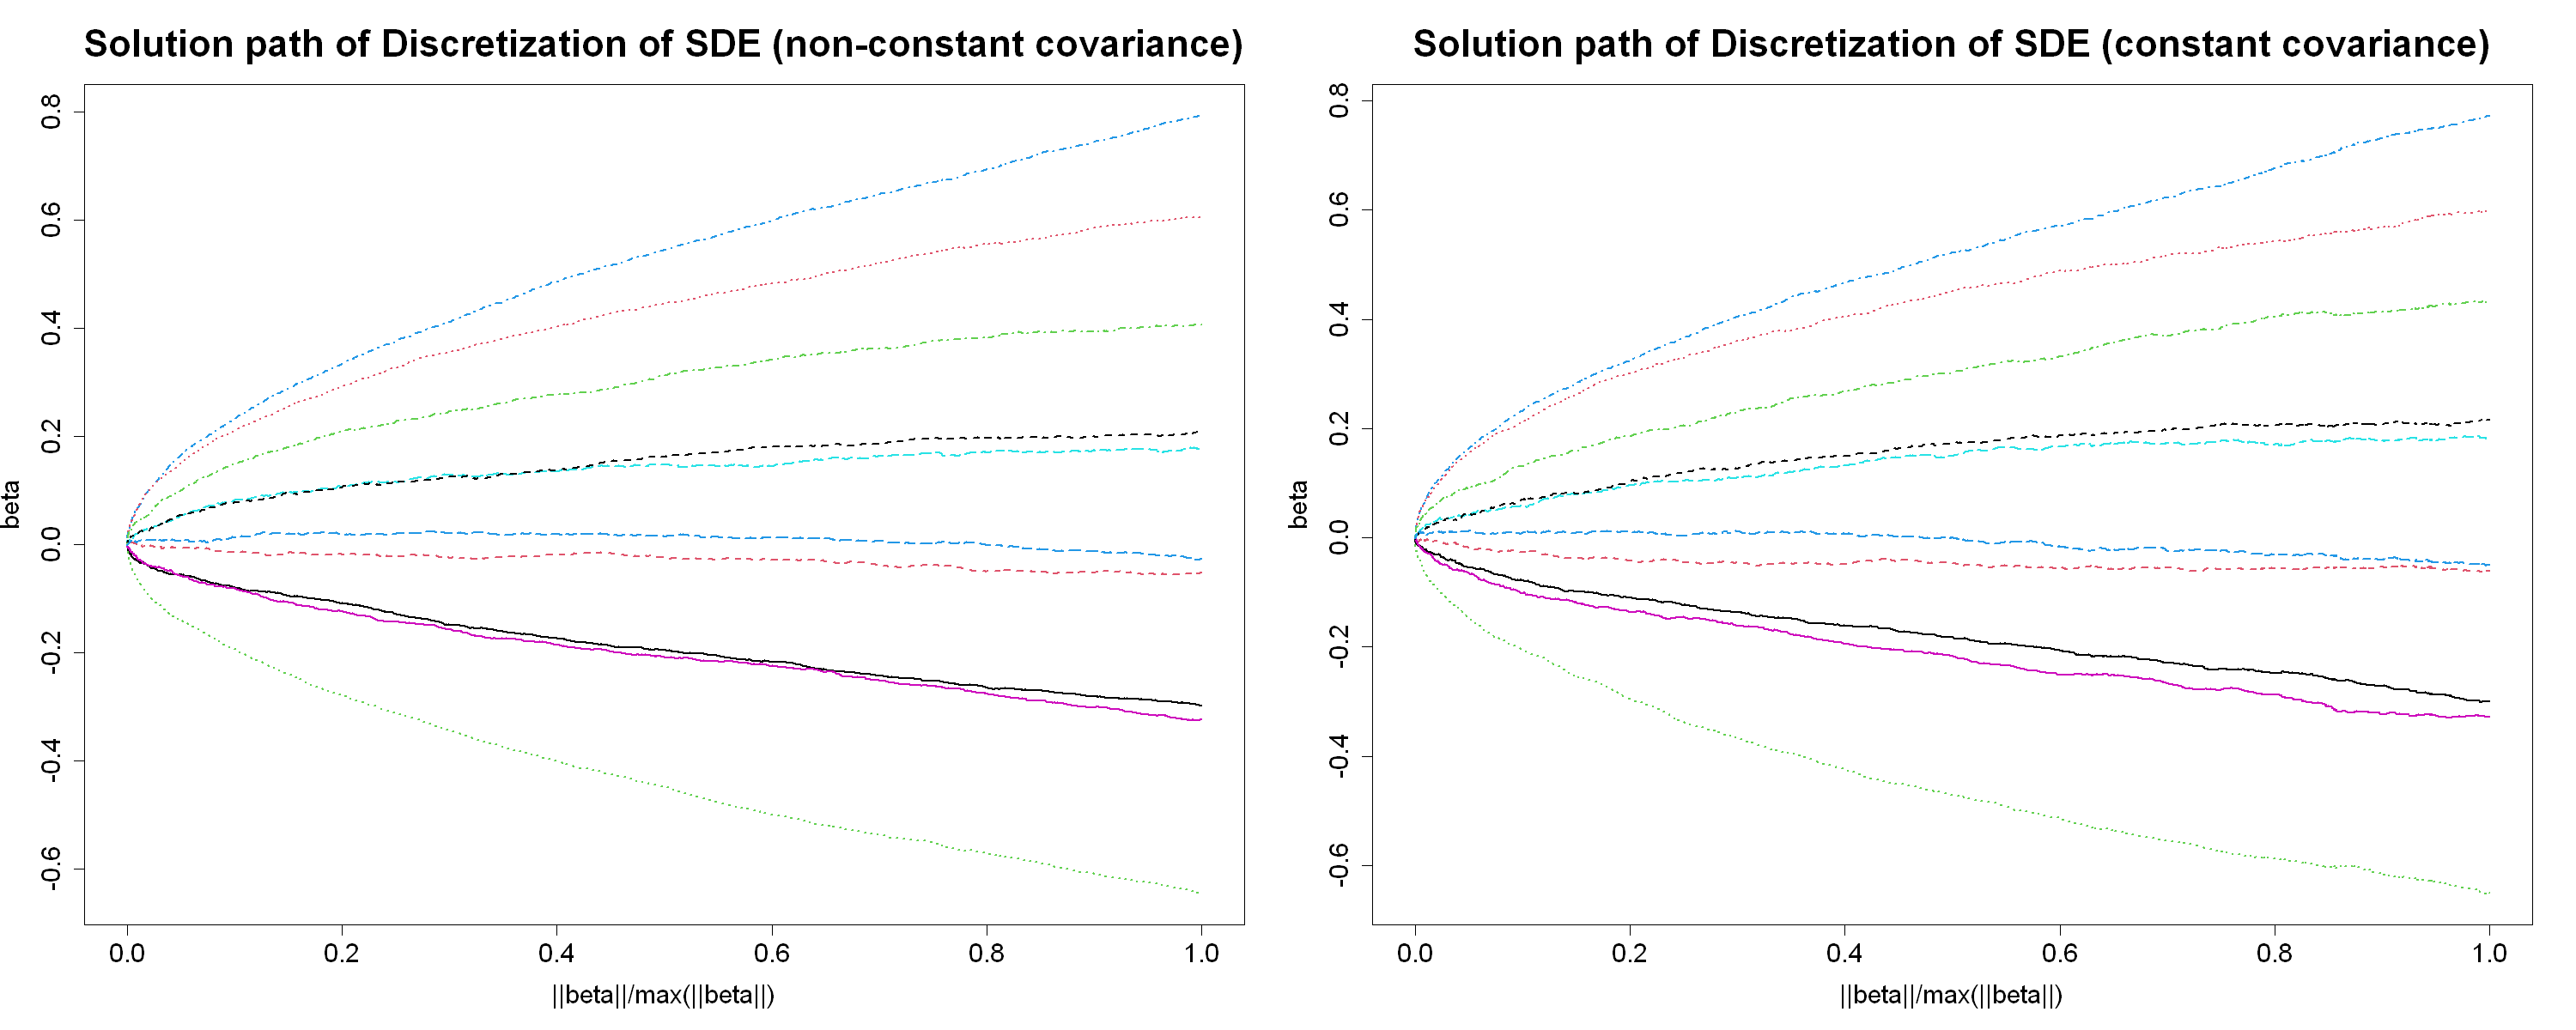
\includegraphics[width=1\linewidth]{fig3.png}
\caption{Discrete solutions of SDE}
\label{fig:Discrete_sde}
\end{figure}

\begin{figure}[h]
\centering
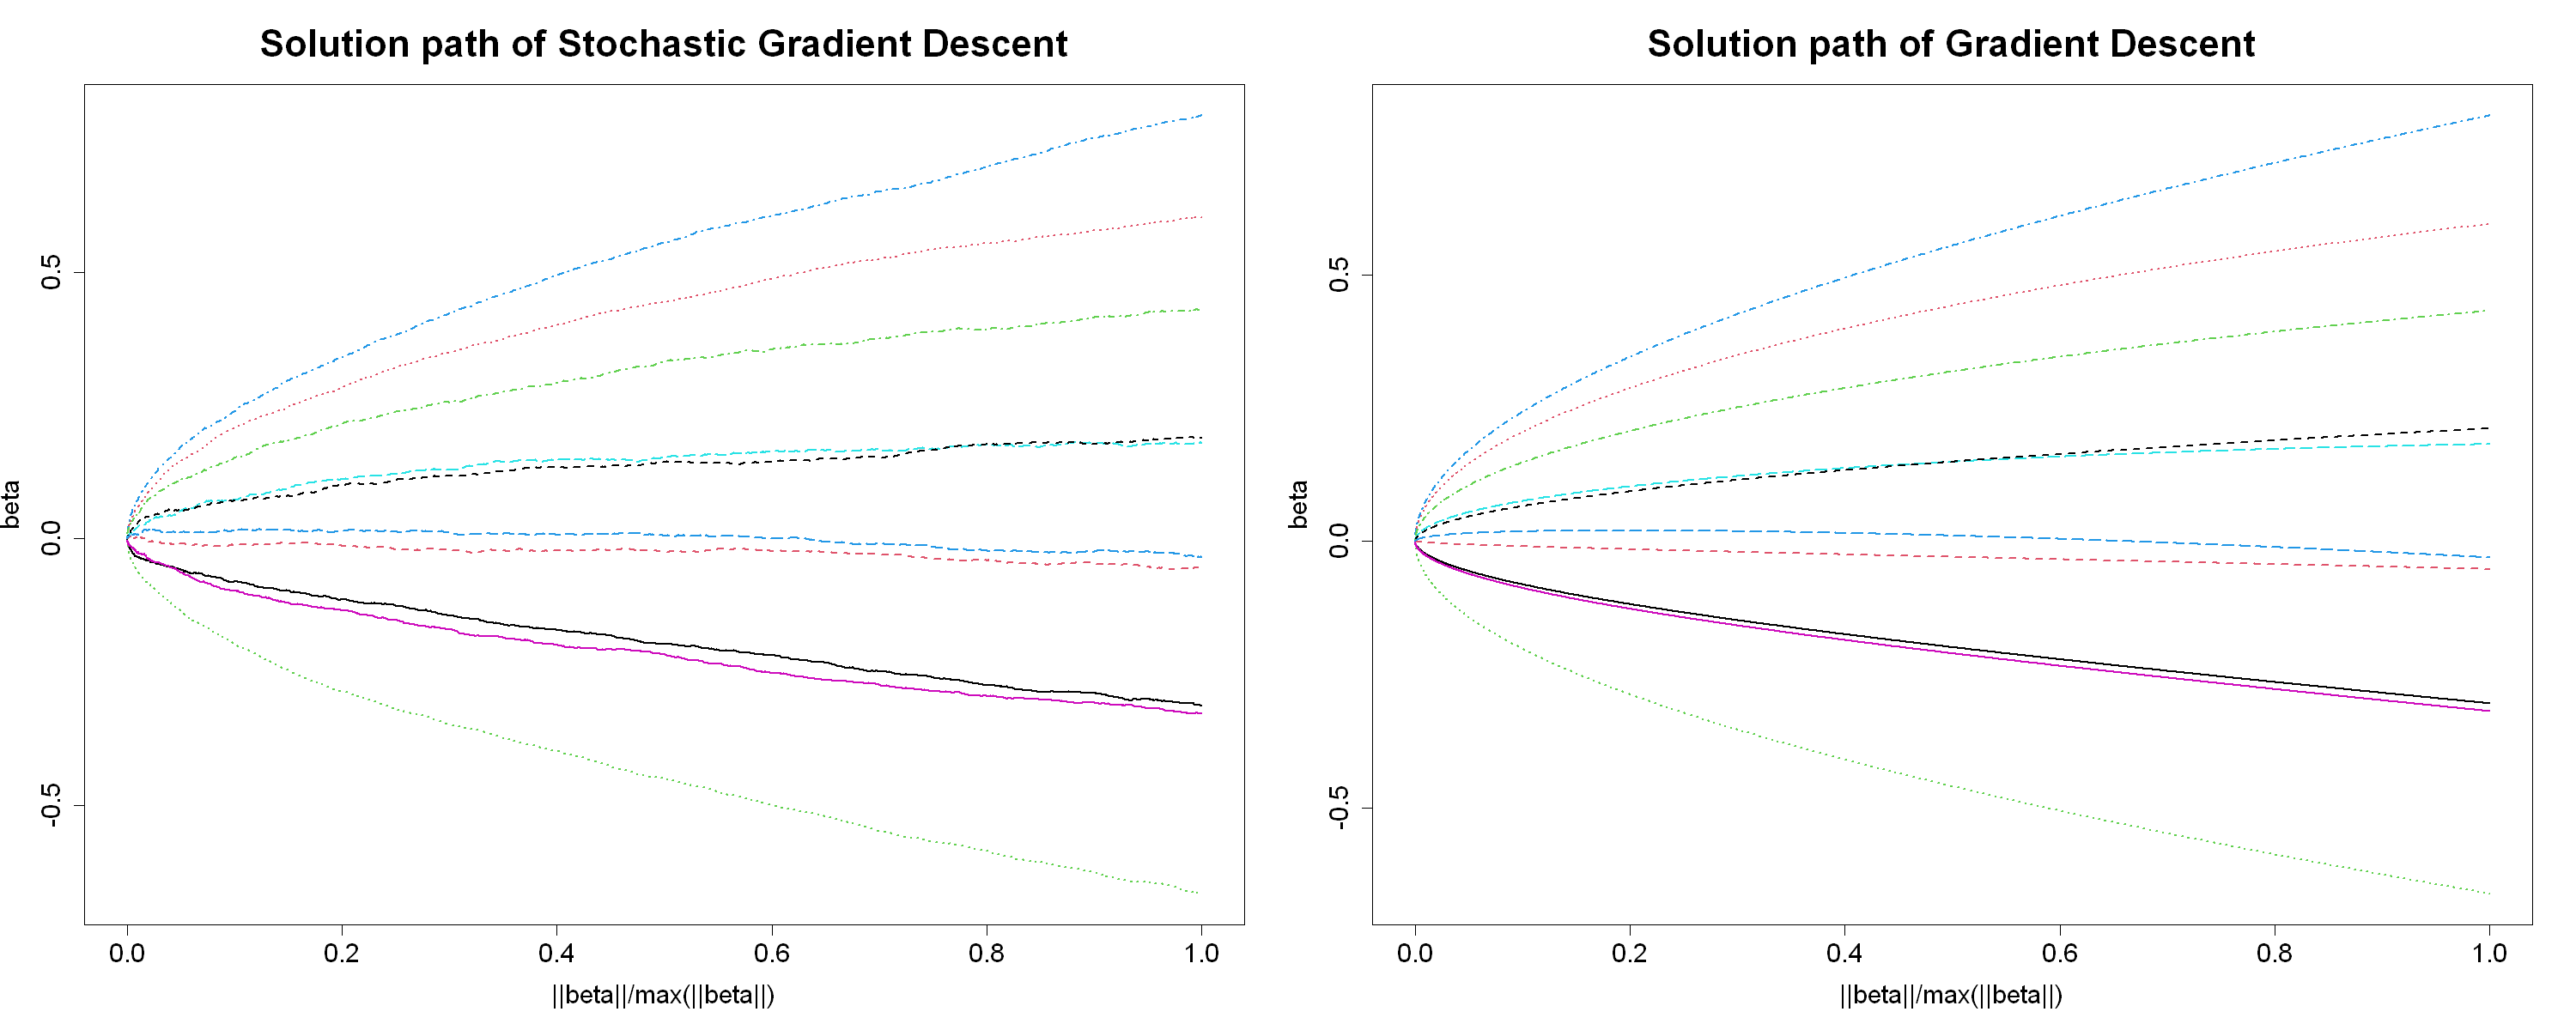
\includegraphics[width=1\linewidth]{fig4.png}
\caption{Stochastic Gradient Descent and Gradient Descent}
\label{fig:gd}
\end{figure}

\begin{figure}[ht]
\centering
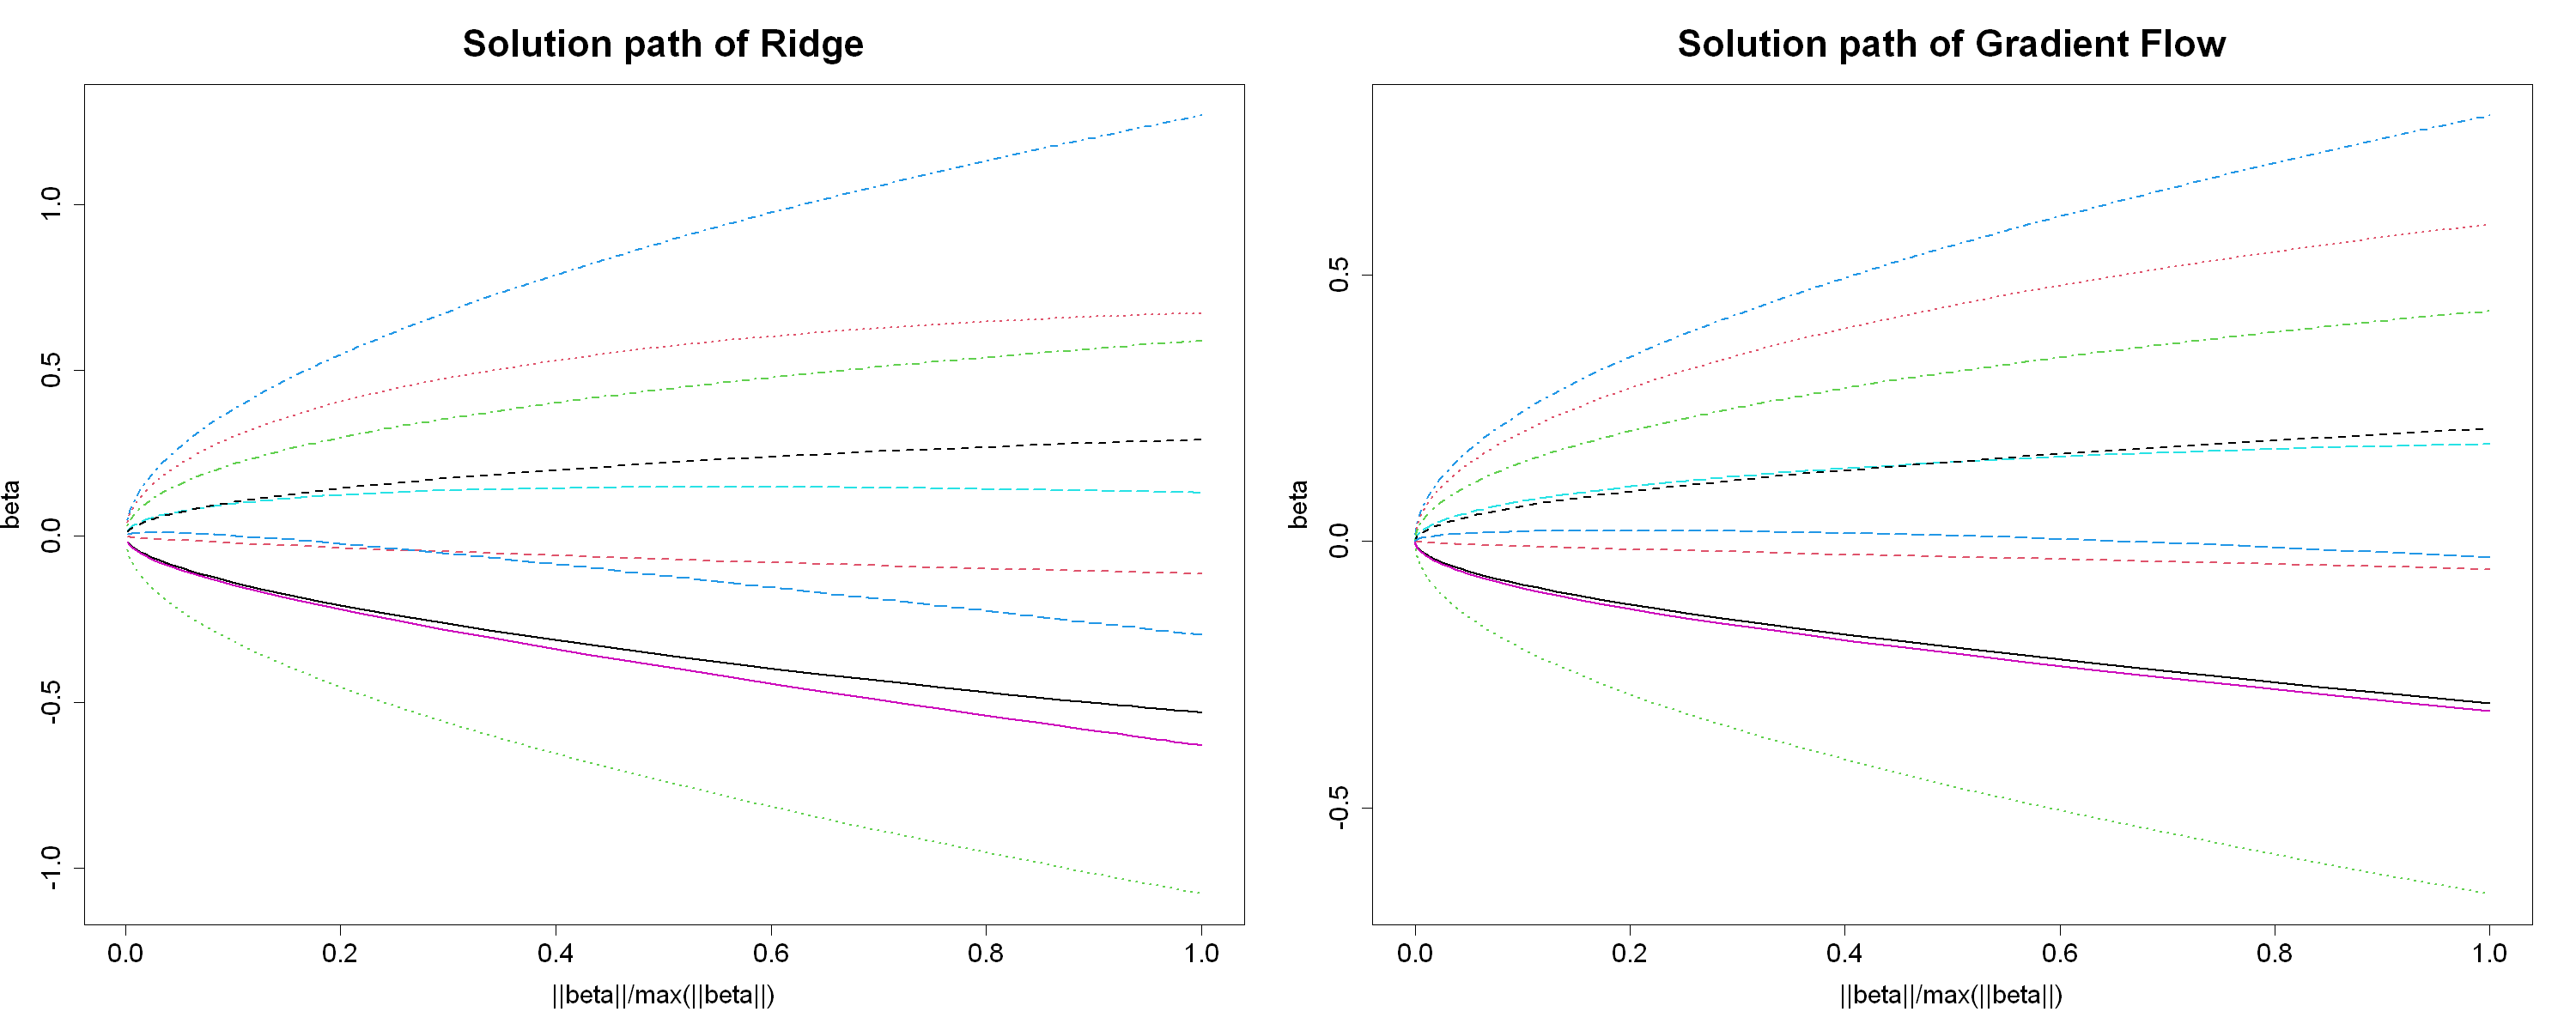
\includegraphics[width=1\linewidth]{fig5.png}
\caption{Ridge Regression and Gradient Flow}
\label{fig:ridge}
\end{figure}

By comparing the simulation results in Figure \ref{fig:Discrete_sde} - \ref{fig:ridge}, we can find that the paths of the coefficients by different methods look similar. It is not surprising because we already know that the methods are all related. The paths of the Gradient Descent and Gradient Flow are the same. And after adding the mini-batch term into the algorithm, the solution path will have little fluctuations, which can be find in the paths of the discrete solutions of SDE and Stochastic Gradient Descent.

We can also find the amplitude of fluctuation is larger when the SDE use constant covariance than using the non-constant covariance. We will further discuss the phenomenon in Subsection \ref{simu2}.

\subsection{Simulation II} \label{simu2}

In this simulation the dimension of $X$ is set to $p=2$, so that we can visualize the searching path of different methods. We set the number of observations $n=200$ and $\sigma^2_{\beta} = 0.3$, $\sigma^2_{n} = 0.1$.

\begin{figure}[p]
\centering
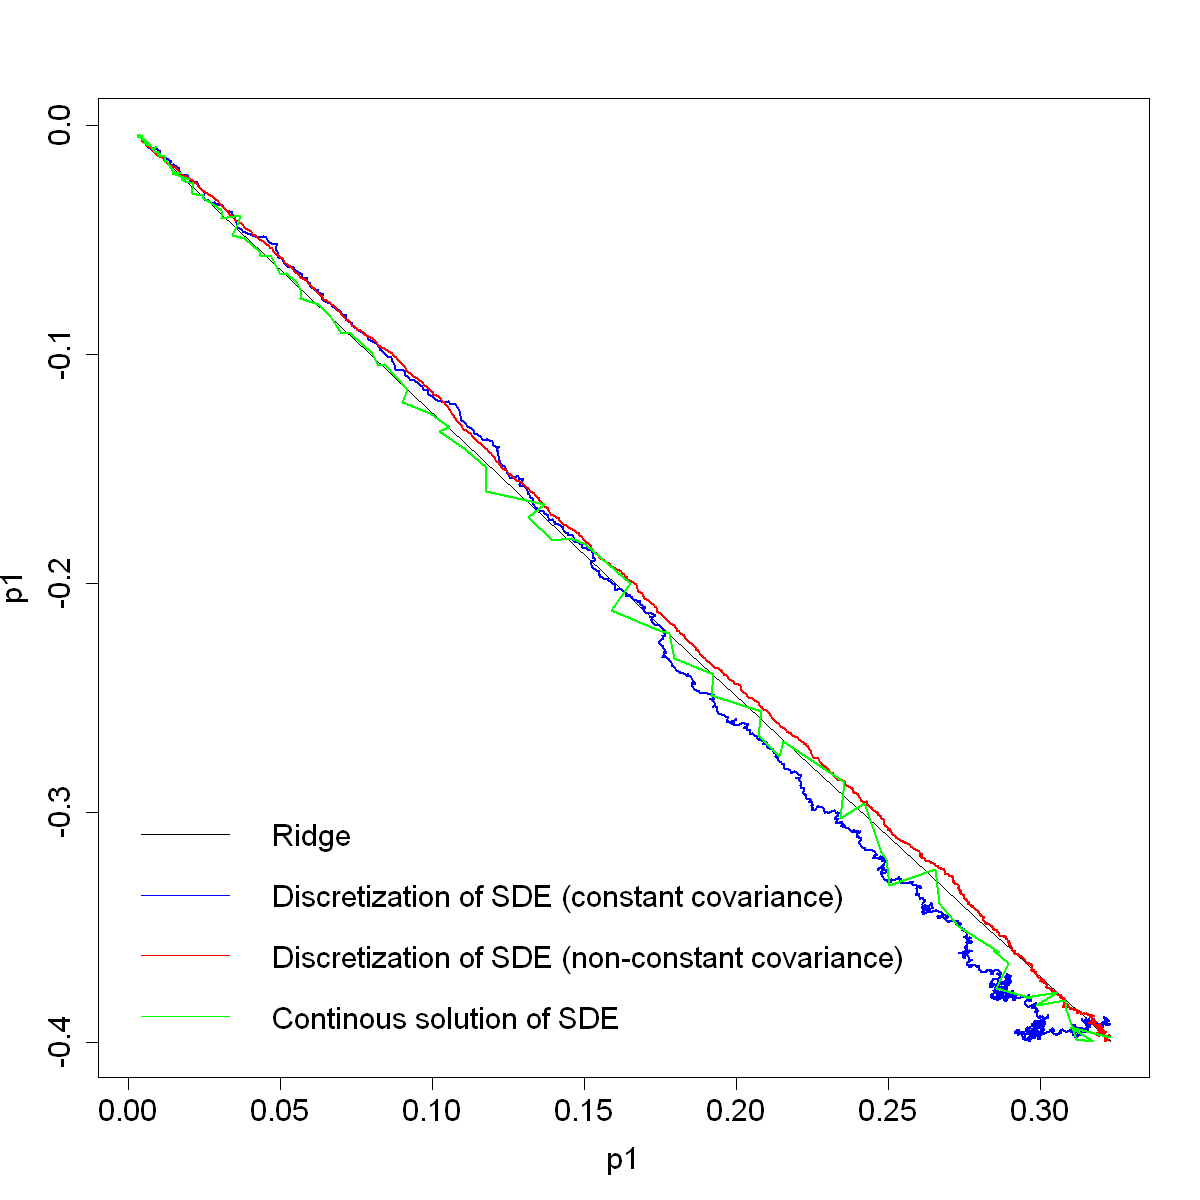
\includegraphics[width=1\linewidth]{fig6.png}
\caption{Searching paths of different methods}
\label{fig:search}
\end{figure}

Figure \ref{fig:search} below shows the results of Ridge Regression, continuous solution of SDE and two discrete solutions of SDE. We can find that continuous solution and discrete solution using the non-constant covariance generally follows the search path of Ridge Regression. This may be because of the non-constant covariance will adaptively control the learning rate of the algorithm.

If we further extend the number of iterations ($nt$, $nk$ or $nlam$), the searching path of SDE with constant covariance will keep changing around the true coefficient $\beta$. From my perspective, it may be explained using the early stopping property of these kinds of methods. The constant convariance is just estimated from $X^TX/n$, which is not related to Mini-batch data. Thus, the discrete solution with constant covariance is just like the Gradient Descent without the $l_2$ norm.

\subsection{Simulation III}

We only implement the risk bounds because I have not figured out how to approximate the coefficient bounds of SGF. I use the result of Ridge Regression to calculate the risk bounds of SGF as Equation \ref{eq:bound}.

\begin{equation}
    \operatorname{Bias}^{2}\left(\hat{\beta}^{\text {ridge }}(1 / t) ; \beta_{0}\right) = \left[\left[\left(X^{\top} X+\lambda I\right)^{-1}-\left(X^{\top} X\right)^{-1}\right] X^{\top} X \beta\right]^2
\end{equation}

\begin{equation}
    \operatorname{Var}_{\eta}\left(\hat{\beta}^{\text {ridge }}(1 / t)\right) = \sigma_n^{2}\left(X^{\top} X+\lambda I\right)^{-1} X^{\top} X\left(X^{\top} X+\lambda I\right)^{-1}
\end{equation}

We generate $X=\Sigma^{1 / 2} W$ without response, and $W$ is drawn from Gaussian distribution. All the diagonal matrices on $\Sigma^{1 / 2}$ is 1 and all the other matrices equal to $\rho$.
The results can be found in the Figure \ref{fig:rou0} and \ref{fig:rou0.5} below. We can find that the of Ridge Regression and GF (together with SGD and SD) will finally converge the same value, while the risk of our SGF will be higher than these methods.

\begin{figure}[h]
\centering
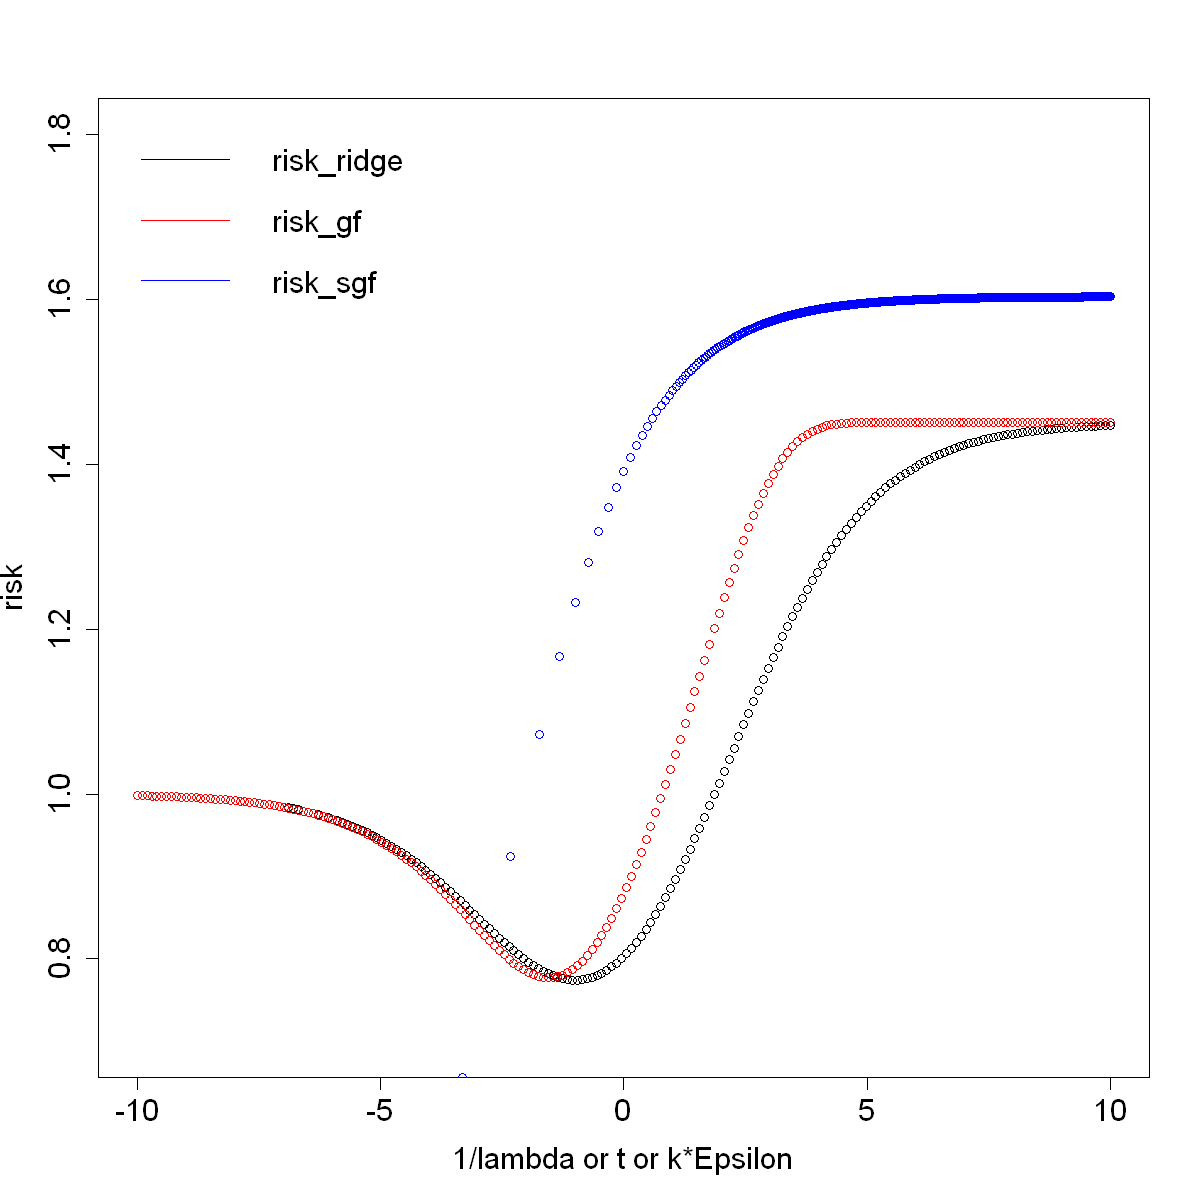
\includegraphics[width=0.9\linewidth]{fig8.png}
\caption{Risk bounds when using Gaussian distribution, rho=0}
\label{fig:rou0}
\end{figure}

\begin{figure}[H]
\centering
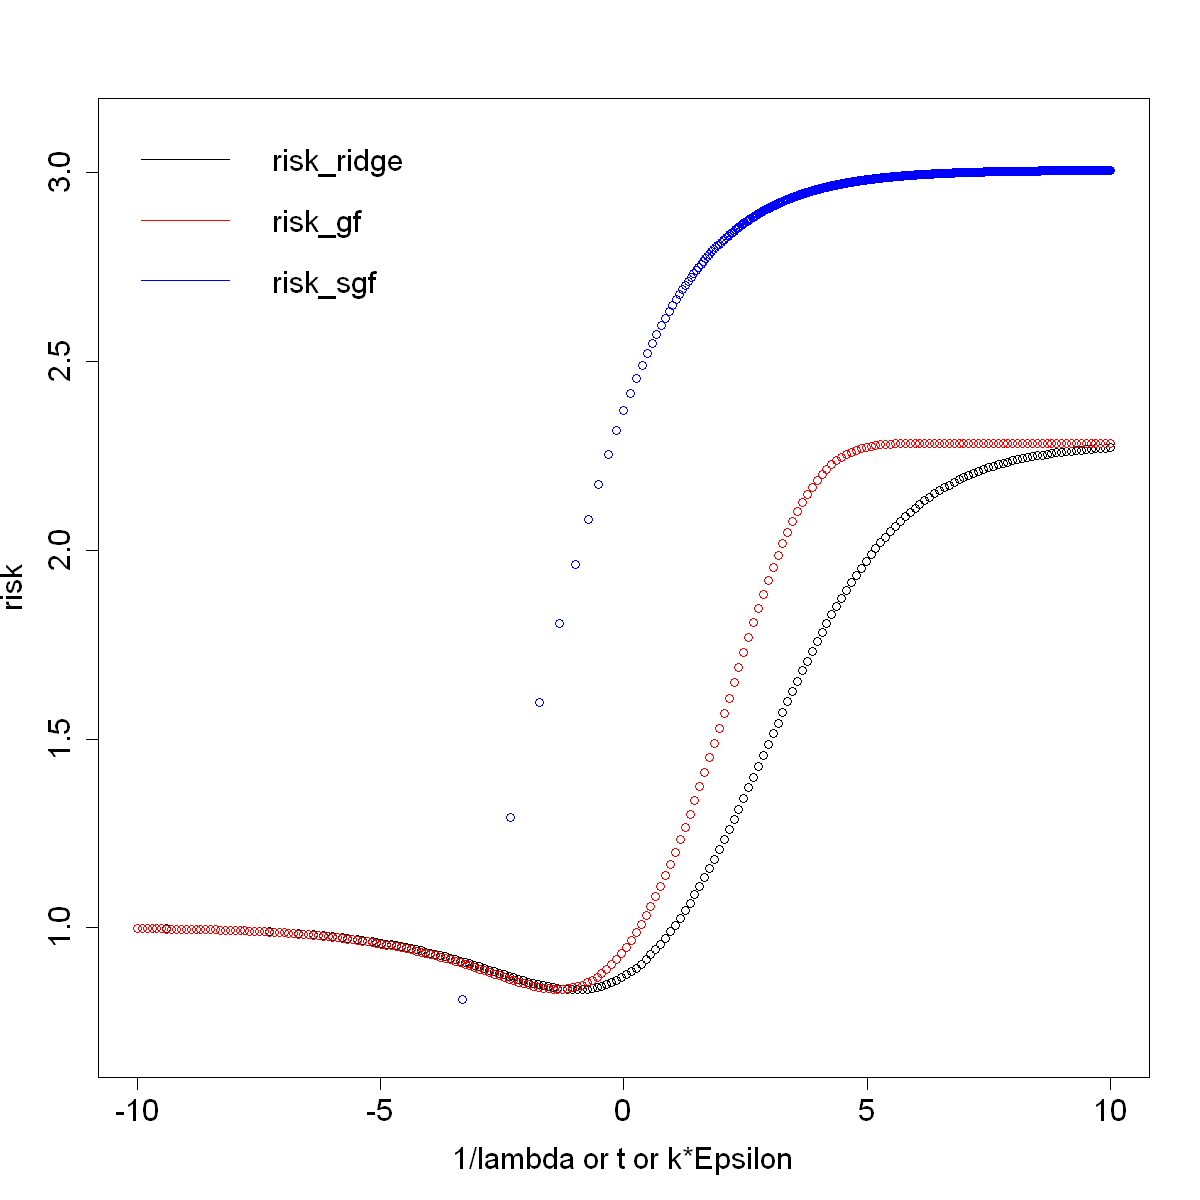
\includegraphics[width=0.9\linewidth]{fig9.png}
\caption{Risk bounds when using Gaussian distribution, rho=0.5}
\label{fig:rou0.5}
\end{figure}

\newpage

\section{Conclusion}

In conlusion, we can find that all these methods we learned in the class and in this paper are highly related. The solution path of them are similar. However, different ways to introduce the stochastic term and the regularization will influence their performance facing different settings of data.

\section{Originality of My Project}
	
In this section, I will post the place to find my code and the originality of the project.

The codes, pictures and my latex files can be found at 

\href{https://github.com/carlosfel/math5472-project}{https://github.com/carlosfel/math5472-project}

The formulas in Section \ref{Summary} are reorganized from \cite{ali2020implicit} and \cite{ali2019continuous}. The final formula of Equation \ref{eq:10}, \ref{eq:12}, \ref{eq:cov} are derived by myself. 

The code to draw the first 5 figures is based on the Solution to the Assignment 2 of MATH5472. The idea and code to implement the GF is based on the Solution to the Assignment 2 of MATH5472. The code to implement the algorithms, including the continuous SGF and two discrete solutions of SDE, is written by me. The code to implement the simulations is written by me.

\bibliographystyle{plain}
\bibliography{reference}

\end{document}